\documentclass[journal]{IEEEtran}
\usepackage{fontspec}
\setmainfont{texgyretermes}[Extension=.otf,UprightFont=*-regular,BoldFont=*-bold,
  ItalicFont=*-italic,BoldItalicFont=*-bolditalic]
\usepackage{unicode-math}
\setmathfont{texgyretermes-math.otf}
\usepackage{graphicx}
\usepackage{booktabs}
\usepackage{cite}
\usepackage{url}
\usepackage{siunitx}
\sisetup{detect-all,per-mode=symbol}

\begin{document}

\title{When Does a KV Memory Tier Pay?\\A First-Order Model for LLM Serving}

\author{Romyull~Islam
\thanks{Manuscript draft, October 2026. R.~Islam is with Kennesaw State University, Kennesaw, GA,
USA (e-mail: mislam22@students.kennesaw.edu).}}% department to be added
\markboth{Draft}{Islam: When Does a KV Memory Tier Pay?}
\maketitle

\begin{abstract}
KV-cache tiers in host memory, SSD and CXL now ship in vLLM, LMCache and NVIDIA Dynamo, yet
reported effects range from none to 5.8$\times$. We give a first-order model of what a tier is
worth: its gain grows with the tokens a workload recomputes per token it generates, $R$, and
saturates at the ratio of recompute to load cost. On real vLLM with its CPU tier, four models of
three architectures and two benchmarks, it predicts measured gains of 6\% to 372\% to within $-2$
to $+15\%$ when recompute is timed alongside decoding. We then apply it to preempted requests, 30 to
99\% of requests in saturated reasoning serving. In seven simulated deployments a decoded token
costs 4 to 30 recomputed ones and first-come-first-served preemption keeps $R$ below 0.9, so a tier
for preempted KV adds only 2 to 10\% to saturation throughput, nothing to goodput at usable latency
targets, and fits in host DRAM except for offline best-of-$N$ batches.
\end{abstract}

\begin{IEEEkeywords}
LLM serving, KV cache, memory tiering, CXL, preemption, performance modeling
\end{IEEEkeywords}

\section{Introduction}
Memory tiers for the KV cache have become products. vLLM's offloading connector and
LMCache~\cite{lmcache} keep KV in host memory, NVIDIA Dynamo adds SSD and remote
tiers~\cite{dynamo_kvbm}, and CXL memory pools are offered as the next
tier~\cite{samsung_cmmd,tang_cxl}. Their reported value ranges from none to 5.8$\times$. A CXL pool
used by LMCache sustains 354K tokens/s on document questions where 512\,GB of DRAM alone falls to
61K, a 5.8$\times$ gain~\cite{samsung_cmmd}; Tang et al.\ report a 30\% larger
batch~\cite{tang_cxl}; on one coding-agent workload, EfficientAgent finds that offloading speeds up one deployment, slows
another and changes nothing on a third~\cite{efficientagent}; and
vLLM recomputes preempted requests by default, its authors having found recomputation comparable to
swapping at the default block size~\cite{vllm}.

Reasoning outputs are long and heavy-tailed: on a production reasoning trace from
Qwen-Bailian~\cite{bailian} the median output is 1.7K tokens, the 99th percentile 35K, and the 10\%
of requests with the longest outputs hold 69\% of the KV byte-seconds. KV memory, not compute,
limits throughput~\cite{kinetics} and the batch~\cite{infscaling}, and requests that outgrow it are
preempted: in our saturation runs 30 to 99\% of requests are preempted. Keeping preempted KV in host memory was proposed in
InferCept, FastServe and CacheOPT~\cite{infercept,fastserve,cacheopt}; vLLM's CPU tier now restores preempted requests, and CXL
is proposed for the same role~\cite{samsung_cmmd}.

\begin{figure}[t]
\centering
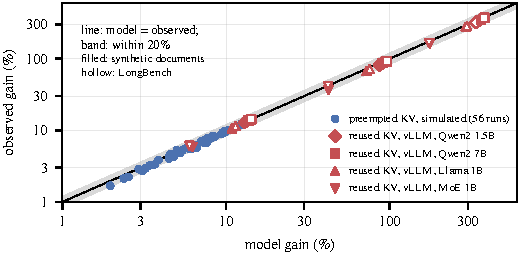
\includegraphics[width=\columnwidth]{fig_teaser.pdf}
\caption{Observed against model-predicted throughput gain of a KV tier. Blue: 56 simulated
saturation runs of preempted KV (seven deployments, FlashAttention-3 and -2 calibrations). Red: real
vLLM with its CPU tier, four models, two benchmarks, $c_r$ measured alongside decoding.}
\label{fig:teaser}
\end{figure}

One quantity separates these cases: the tokens a workload recomputes per token it generates, $R$.
When $R$ is in the thousands, as when a 48K-token
document is recomputed for a 2-token answer, the tier multiplies throughput, up to the ratio of
recompute to load cost. When $R$ is below one, as for preempted requests, the gain cannot exceed
$R$ divided by the cost of a decoded token in recomputed tokens, $\rho$, which compute-bound
prefill makes 4 to 30 in the deployments we simulate.
This letter contributes:
\begin{itemize}
\item a first-order model of a KV tier's throughput gain (Section~\ref{sec:model});
\item its test on real vLLM with four models of three architectures and two benchmarks, from $R=7$
to 1,027 (Section~\ref{sec:real});
\item simulations of $R$, $\rho$, the gain and the tier capacity for preempted KV in reasoning
serving over seven deployments, validated against LLMServingSim and vLLM (Section~\ref{sec:preempt});
\item the conditions under which a tier for preempted KV would pay (Section~\ref{sec:pays}).
\end{itemize}

\section{A First-Order Model}
\label{sec:model}
Let $c_d$ be the GPU time per generated token when nothing is recomputed, $c_r$ the time to
recompute one token and $c_l$ the GPU time to load one from the tier. If a workload recomputes $R$
tokens per generated token, a tier that keeps them changes the time per generated token from
$c_d+Rc_r$ to $c_d+Rc_l$, so throughput at saturation rises by
\begin{equation}
g = \frac{R\,(c_r-c_l)}{c_d+R\,c_l}.
\label{eq:gain}
\end{equation}
With $\rho=c_d/c_r$, $g\approx R/\rho$ when $Rc_l\ll c_d$ and $c_l\ll c_r$, and $g$ approaches
$c_r/c_l-1$ when $Rc_l\gg c_d$, that is $R\gg\rho\,c_r/c_l$: then the tier's bandwidth, not its
capacity, decides the gain. With $c_l=0$ (an ideal tier) $g=R/\rho$ is an upper bound.

\textbf{Why $\rho$ is large.} A decode step reads the weights and every running request's KV from
HBM, and with the KV cache full it reads all of it, so $c_d \approx (W + K)/(B \cdot
\mathrm{BW})$ for weights $W$, KV $K$ and batch $B$. Recompute is a prefill: $2P$ FLOPs per token for
$P$ parameters plus attention, executed compute-bound. For a 70B model on 8 H100 GPUs $\rho$ is 7 to 15.

\textbf{Why $R$ is small for preemption.} vLLM puts a preempted request at the head of the waiting
queue, and part of its KV is still in the GPU prefix cache when it resumes: 10 to 53\% of resumed
tokens in our runs. Even with 90\% of requests preempted, 4 to 9 times each on average in
best-of-$N$ batches, $R$ stays below 0.9, so the gain in our runs is bounded by $0.9/\rho$.

\textbf{Published gains.} Samsung's benchmark asks 2-token questions about 48K-token
documents~\cite{samsung_cmmd}, so every miss recomputes 24,000 tokens per generated token and the
gain is bounded by $c_r/c_l-1$ rather than by $R$. Tang et al.'s 30\% larger batch at the same
time-to-first-token target with a CXL prefix-KV store~\cite{tang_cxl} is also a case of reused prefixes.

\section{Test on Real vLLM}
\label{sec:real}
We test Eq.~\ref{eq:gain} with vLLM 0.31 and its native CPU tier~\cite{vllmblog} on an RTX 4500 Ada, GPU cache fixed
at 32K tokens, with four models of three architectures: DeepSeek-R1-Distill-Qwen 1.5B and 7B
(Qwen2), Llama-3.2-1B and Granite-3.1-1B-A400M (mixture of experts, 8 of 32 experts per token). Two
benchmarks of 16 documents, 8 questions each: synthetic 4,096-token documents, and LongBench
documents of 2,048 to 6,144 tokens from five tasks with their real questions. All requests arrive at
once in round-robin order, so a document's KV leaves the GPU before its next question; answers of 4,
64 and 512 tokens set $R$ (7 to 1,027). Recomputing and offloading runs use the same GPU cache, and
the CPU tier holds all documents. $c_r$ (\SIrange{16}{129}{\micro\second}) comes from a separate
prefill microbenchmark, interpolated to each document's length; $c_l$ (\SIrange{1.2}{2.4}{\micro\second})
is the KV bytes per token over the measured 21.6 to \SI{24.0}{\giga\byte\per\second} pinned
host-to-GPU bandwidth; $c_d$ comes from the offloading run.

Over two or three repetitions (spread at most 2.2\%, 17\% for 4-token answers) the model
over-predicts in all 24 cases, by 4 to 12\% on the dense models and 17 to 33\% on the mixture of
experts (Table~\ref{tab:reuse}). The error is in $c_r$: here recompute shares steps with decoding
requests, which already read the weights. Measured that way, as the time 16 extra 4,096-token
prefills add to 7 decoding requests, $c_r$ is 3 to 5\% lower on the dense models and 12 to 14\%
lower on the mixture of experts, and the error is $-2$ to $+8\%$ in 23 of 24 cases and $+15\%$ in
one. $\rho$ is 48 to 309 because $c_d$ includes each document's first prefill, spread over 4 to 512
answer tokens, and the GPU cache holds at most 7 requests.

\begin{table}[t]
\centering
\caption{Real vLLM: gain of the CPU tier over recomputation for answers of 4, 64 and 512 tokens,
and the model's error with $c_r$ measured alone or alongside decoding.}
\label{tab:reuse}
\footnotesize
\setlength{\tabcolsep}{4pt}
\begin{tabular}{llrrr}
\toprule
 & & measured gain (\%) & \multicolumn{2}{c}{error (\%), $c_r$ timed} \\
model & bench & 4 / 64 / 512 tokens & alone & with decoding \\
\midrule
Qwen2 1.5B & synth. & 342 / 82 / 13 & +6 to +11 & +1 to +6 \\
Qwen2 1.5B & LongB. & 321 / 88 / 13 & +5 to +11 & $-$1 to +5 \\
Qwen2 7B & synth. & 348 / 87 / 14 & +4 to +8 & 0 to +4 \\
Qwen2 7B & LongB. & 372 / 92 / 14 & +5 to +9 & +1 to +4 \\
Llama 1B & synth. & 276 / 67 / 11 & +6 to +12 & +2 to +8 \\
Llama 1B & LongB. & 285 / 72 / 11 & +4 to +10 & 0 to +5 \\
MoE 1B & synth. & 163 / 37 / 6 & +24 to +33 & +7 to +15 \\
MoE 1B & LongB. & 166 / 42 / 6 & +17 to +24 & $-$2 to +5 \\
\bottomrule
\end{tabular}

\end{table}

\section{Preempted KV in Reasoning Serving}
\label{sec:preempt}
\subsection{Setup}
\textbf{Simulator.} A step-level simulator follows vLLM V1's scheduler: running requests are served
in admission order, the last one is preempted when a block is missing, and preempted requests resume
first; freed blocks stay in the prefix cache until reused. Tier policies: swap on preemption, and
write-through with LRU eviction as in vLLM's CPU offloading connector. Step times come from a
roofline whose efficiencies are fitted to Vidur's measured kernel profiles~\cite{vidur}: whole-layer
error 4 to 10\% median on H100 (Llama-2-70B, held-out CodeLlama-34B) and 4 to 7\% on A100
(Llama-3-70B, held-out Llama-3-8B, contexts to 16K). Prefill attention uses FlashAttention-3
efficiency~\cite{fa3} or, as a pessimistic case that makes recompute dearer, the measured
FlashAttention-2 curve.

\textbf{Validation.} Against LLMServingSim 2.0~\cite{llmservingsim2}, an independent port of vLLM's
scheduler with its own GPU profiles, on 64 requests with 10K to 30K-token outputs: preemptions 50 vs
50, recomputed tokens within 0.3\% with GPU prefix-cache reuse disabled as in LLMServingSim, and
per-request finish times correlated at 0.9999 with a 14\% median timing offset. Against real vLLM
0.31 (Qwen2.5-0.5B, KV fixed at 4,096 blocks, the first 300 Bailian requests with prompts scaled by
1/8 and outputs by 1/4): 297 vs 277 preemptions and 111K vs 118K recomputed tokens. With
DeepSeek-R1-Distill-Qwen-1.5B on 400 Bailian requests: 275 vs 270 preemptions, 569K vs 574K tokens.

\textbf{Workloads and deployments.} The Bailian reasoning trace (10,812 requests) and best-of-1, 16
and 64 groups of MathArena AIME 2025 outputs from the model with the matching
architecture~\cite{matharena} (each group resamples the four recorded outputs per problem).
Saturation and capacity runs submit every request at once; online runs use the trace's arrivals.
Llama-70B on 8 H100, H200 and B200; QwQ-32B on 2 and 4 H100; Qwen3-235B FP8 on 8 H100; DeepSeek-R1
FP8 on 8 H200, whose replicated MLA latent holds only 0.56M tokens. vLLM defaults: block 16, up to
1,024 running requests, 8,192 tokens per step.

\subsection{Results}
\begin{figure}[t]
\centering
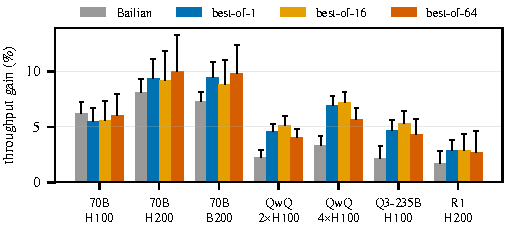
\includegraphics[width=\columnwidth]{fig_gain.pdf}
\caption{Saturation throughput gain of keeping preempted KV (unlimited tier) over recomputing it;
bars use FlashAttention-3 efficiency, whiskers the FlashAttention-2 calibration.}
\label{fig:gain}
\end{figure}

\textbf{Saturation.} With every request submitted at once, the regime with the most preemption,
keeping preempted KV raises throughput by 2 to 10\% (median 5.5\%) and by at most 13\% with the
pessimistic prefill calibration (Fig.~\ref{fig:gain}). The simulated gains match $R/\rho$, with
$c_d$ and $c_r$ taken from each recompute run, with correlation 0.997 and a mean absolute error of
0.3 points (at most 0.9; Fig.~\ref{fig:teaser}). The gain is largest for 70B on H200 and B200, whose
larger batches make decode cheaper per token, and smallest for DeepSeek-R1.

\textbf{Admission tuning.} Lowering vLLM's running-request limit from 1,024 to the best value (96 to
192, 512 for DeepSeek-R1) recovers 0 to 6\% by itself in four deployments; over the best-tuned
recompute baseline an unlimited tier adds 1.7 to 5.9\% with BF16 KV and 5 to 8\% with FP8 KV (70B,
best-of-$N$), the most favorable case we found, because FP8 halves the KV bytes read per decode step
and so cuts $\rho$ by 44 to 49\%.

\textbf{Online load.} With Bailian arrivals the gain is zero below saturation; best-of-16 arrivals
saturate the recompute baseline below the offline rate, and at 0.85 to 0.95 of it the tier adds up
to 6.4\%. Goodput, the highest load that keeps the 99th-percentile time to first token under 10 or
60\,s, is unchanged in 19 of 20 cases.

\begin{figure}[t]
\centering
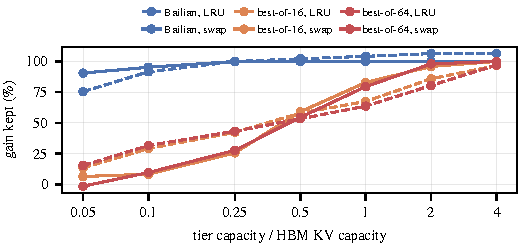
\includegraphics[width=\columnwidth]{fig_capacity.pdf}
\caption{Share of the unlimited tier's gain kept as tier capacity grows (median over 70B on H100 and
H200, QwQ-32B and DeepSeek-R1). LRU: write-through with LRU eviction.}
\label{fig:cap}
\end{figure}

\textbf{Capacity.} For the Bailian trace, even submitted all at once, a swap tier of 0.1 to 0.25
times the HBM KV capacity keeps 93 to 100\% of the gain (Fig.~\ref{fig:cap}); with its real
arrivals the tier peaks at 62\,GB. Only best-of-$N$ batches submitted at once need 1 to 2 times the
HBM KV with swap and 2 to 4 times with LRU write-through, up to 3.4\,TB for 70B on 8 H200 GPUs,
against 2\,TB of DRAM in a DGX node. Pooling eight nodes' tiers saves 49 to 64\% of capacity, but the
pooled peak (at most 1.3\,TB) is a twelfth of the eight nodes' 16\,TB of DRAM, so capacity beyond host DRAM is
not needed.

\textbf{Real system.} On real vLLM with Qwen2.5-0.5B, removing the memory pressure altogether raised
throughput by only 5.9\%, and vLLM's native CPU tier lowered it by 3.9\%: it cut recomputation by
only 34\% while writing KV through to the CPU. With DeepSeek-R1-Distill-Qwen-1.5B, preemption gave
$R=0.43$ against $\rho$ = 23 to 128 at 2K to 16K tokens of context, so $R/\rho$ bounds the gain at 2\%.

\section{When Does a Tier Pay?}
\label{sec:pays}
The model points to three ways a KV tier becomes worth its memory. First, cheaper decode lowers
$\rho$: FP8 or INT4 KV halves or quarters the bytes read per decode step, and larger HBM allows larger
batches; with FP8 KV our gain over tuned admission rises to 5 to 8\%. Second, schedulers that preempt on purpose raise $R$:
a latency-oriented scheduler that time-slices long requests, as in skip-join multi-level
feedback~\cite{fastserve}, would recompute the same context at every slice without a tier, so $R$ can
exceed 1; FastServe pairs its scheduler with host-memory KV. Third, workloads whose prompts dwarf
their outputs raise $R$: document questions~\cite{samsung_cmmd} and agents whose context is evicted
while they wait for a tool and is recomputed for a short next turn~\cite{efficientagent,unison}. For
preempted KV under first-come-first-served admission none of these holds: over-admission rather
than missing capacity causes the recomputation, and a better admission limit removes part of it at
no cost. An operator can check a deployment with three ratios: $R$, the scheduled tokens beyond
prompt and output tokens per output token; $\rho$, from a short microbenchmark like the one above;
and $c_l/c_r$, from the tier's bandwidth.

\section{Related Work and Limitations}
That a decoded token costs 16.7 to 200 times a prefilled one at small batch is
known~\cite{sarathi} and underlies phase splitting~\cite{splitwise,distserve}. Prior work
characterizes the memory wall of reasoning~\cite{kinetics,infscaling}, tiers decoding KV
by sparse attention or token importance~\cite{oasiskv,notallthoughts}, manages memory for tree
search~\cite{fasttts}, models preemption from length distributions~\cite{congestion}, measures
preemption in RL rollouts~\cite{rollpacker}, and sets KV reservations under length
uncertainty~\cite{robustkv}. Per-request choices between swapping and recomputing are weighed by
InferCept and restore-or-recompute models~\cite{infercept,restore_recompute}, CacheFlow plans what to
recompute and what to load to cut restore latency~\cite{cacheflow}, measurements in vLLM locate the
break-even prefix length~\cite{pykvcache}, Meng et al.\ give the cached-to-new token ratio at which
prefill becomes transfer-bound~\cite{mengoffload}, and Li et al.\ model the cloud cost of storing KV
for reuse~\cite{licost}. We add a
closed-form, workload-level model of the gain, its test on real vLLM, and measurements of its inputs
for preempted KV in reasoning traffic.

The step-time model is calibrated on profiles up to 4K tokens on H100 (16K on A100) and extrapolated
with the roofline beyond; MLA and MoE timings are not validated against measurements; the preemption
simulations do not model prompts shared across requests. The real-vLLM tests use 1B to 7B models on one GPU (Gemma-3's
sliding-window layers did not fit the fixed GPU cache), and $c_d$ there is taken from the offloading run, so the test checks the recompute and load
terms of Eq.~\ref{eq:gain}, not $c_d$. On the reasoning trace the simulator's LRU tier removes 99.7\% of the recomputed tokens, where
vLLM's removes 43\%, so simulated tier gains are upper bounds.

\section{Conclusion}
A KV tier pays in proportion to the tokens it saves from recomputation per token generated, up to the
ratio of recompute to load cost; on real vLLM, four models and two benchmarks, this predicts gains of 6\%
to 372\% to within $-2$ to $+15\%$ with recompute timed alongside decoding.
For reasoning and test-time-scaling workloads, keeping preempted KV in host DRAM or CXL memory is
worth 2 to 10\% of saturation throughput and nothing at usable latency, because in the deployments
we simulate a recomputed token costs a fourth to a thirtieth of a decoded one and first-come-first-served preemption recomputes
fewer than one token per token generated.

\bibliographystyle{IEEEtran}
\bibliography{p1}

\end{document}
